% arara: pdflatex: { shell: on }
%! arara: pdflatex: { shell: on }
% arara: biber
% arara: pdflatex
% arara: pdflatex
\documentclass[load-preamble+,ngerman,british,american]{cnltx-doc}
\usepackage[utf8]{inputenc}
\usepackage{chemnum}
\setcnltx{
  package = chemnum ,
  info    = numbering of chemical compounds ,
  authors = Clemens Niederberger ,
  email   = contact@mychemistry.eu ,
  url     = https://github.com/cgnieder/chemnum/ ,
  add-cmds = {
    chemnumshowdef,
    chemnumshowref,
    cmpd ,
    initcmpd ,
    labelcmpd ,
    cmpdplain ,
    cmpdproperty ,
    cmpdref ,
    replacecmpd ,
    resetcmpd ,
    setchemnum ,
    cmpdshowdef ,
    cmpdshowref ,
    newcmpdcounterformat ,
    subcmpdplain ,
    submaincmpdplain ,
    subcmpdproperty ,
    subcmpdshowdef ,
    subcmpdshowref ,
  } ,
  add-silent-cmds = {
    arrow,
    bottomrule,
    ch,chemfig,chemname,
      CNlabel,CNlabelnoref,CNlabelsub,CNlabelsubnoref,
      CNref,CNrefsub,CNsubnoref,
      compound,cs,
    declarecompound,definesubmol,detokenize,
    expandfull,expandtwice,
    fcite,
    includegraphics,
    keyis,
    marginnote, midrule,
    NewDocumentCommand,
    schemestart,schemestop,setatomsep,
    theffbibliography, toprule
  } ,
  index-setup = { othercode=\footnotesize,level=\addsec },
  makeindex-setup = { columns=3,columnsep=1em } ,
  add-frame = false
}
\usepackage[artemisia]{textgreek}
\activatechemgreekmapping{textgreek}

\usepackage{chemformula}
\setchemformula{format=\libertineLF}
\usepackage{chemfig,relsize}
\setatomsep{1.78500 em}
\setbondstyle{line width = 0.06642 em}
\renewcommand*\printatom[1]{\textsmaller{\ensuremath{\mathsf{#1}}}}

\usepackage{array,booktabs,csquotes}

\usepackage{graphicx}

\defbibheading{bibliography}[References]{\addsec{#1}}

\usepackage{acro,accsupp}
\acsetup{
  short-format = \scshape ,
  first-style = short
}
\DeclareAcronym{pdf}{
  short = pdf ,
  long  = portable document format ,
  pdfstring = PDF ,
  accsupp = PDF
}
\DeclareAcronym{eps}{
  short = eps ,
  long  = encapsulated postscript ,
  pdfstring = EPS ,
  accsupp = EPS
}
\DeclareAcronym{ps}{
  short = ps ,
  long  = postscript ,
  pdfstring = PS ,
  accsupp = PS
}
\DeclareAcronym{id}{
  short = id ,
  long  = identification key ,
  pdfstring = ID ,
  accsupp = ID
}

\begin{document}
\selectlanguage{american}

\section{License and Requirements}\label{sec:license-requirements}
\license

\chemnum\ requires the bundles \bnd{l3kernel}~\cite{bnd:l3kernel} and
\bnd{l3packages}~\cite{bnd:l3packages}.  It also requires the
\pkg{translations} package~\cite{pkg:translations},
\pkg{chemgreek}~\cite{pkg:chemgreek} and the \pkg{psfrag}~\cite{pkg:psfrag}
package.

\section{News}\label{sec:news}
The \chemnum\ package has been my first attempt to create a comprehensive
labeling package for chemical compounds.  However, it had and has more than
one weakness and its code was -- to be frank -- a mess.  Version~1 is now a
complete re-write of \chemnum\ where I tried to achieve several points:
\begin{itemize}
  \item A cleaner code internally.
  \item A cleaner user interface, \ie, more user macros for different tasks, a
    unified naming of the commands and a less redundant naming of the
    options.
  \item Extended functionality such as sorting and compressing of sublabel
    lists and sorting and merging of main label lists.
\end{itemize}

Although the syntax seems more or less the same at first sight quite a number
of changes have been made that make version~1 incompatible with version~0.
While I thought a while about maintaining backwards compatibility version~0
was known to be in an experimental stage where everything was allowed to be
changed at any time.  So users \emph{could} know there was a risk.  I have a
feeling that many users nevertheless didn't realize this and may be bothered
by this incompatibility.  So I am well aware that the update will
inconvenience some users.  However, since version~0 won't be updated any more
it made more sense to make a breaking update once.

The same is not true for version~1.  The syntax and commands described in this
manual will not be changed as easily and from this version on I will take care
of backwards compatibility.

For those people wanting to keep older versions: they are are still available
from websites such as \website{ctanhg.scharrer-online.de} or
\securewebsite{bitbucket.org/cgnieder/chemnum}.  You can also email me for an
older version.

Many commands have got a new name! The most important ones are:
\begin{itemize}
  \item \cs*{cmpdref}; this is now called \cs{replacecmpd}.
  \item \cs*{cmpdinit}; this is now called \cs{initcmpd}.
  \item \cs*{cmpdreset}; this is now called \cs{resetcmpd}.
  \item \cs*{cmpdsetup}; this is now called \cs{setchemnum}.
\end{itemize}
However, there are many more changes.  Basically all options have new names
and often do their thing slightly different from the way things have been
before.

Please note that this overall change does not mean that version~1 is version~0
declared stable.  It is very likely that version~1 will now have quite a
number of bugs to be fixed and probably missing features, too.  So I'd be very
glad to receive feedback either on \chemnum's homepage
\securewebsite{github.com/cgnieder/chemnum} or via email to
\email{contact@mychemistry.eu}.

\section{Overview over the Available Commands}\label{sec:overv-over-avail}

This section lists all available commands with a brief description.  Commands
marked with \expandablesymbol\ are expandable in an \cs*{edef} like context.
Most of the commands will be explained in a later section in more detail.

\begin{commands}
  \command{cmpd}[\sarg\code{+}\oarg{options}\marg{list of \acp{id}}]
    The main command for creating and refering to compound labels.  This
    command is described in detail in section~\ref{sec:deta-comp-labels}.  For
    many people this will be the only command they need.
  \command{refcmpd}[\oarg{options}\marg{\ac{id}}]
    This command only refers to an already defined label but does not define a
    label itself.  This is an alias of \cs{cmpd}\code{+}.
  \command{labelcmpd}[\oarg{options}\marg{\ac{id}}]
    This command only defines a new label but does not print it.  This is an
    alias of \cs{cmpd}\sarg.
  \expandable\command{cmpdplain}[\marg{\ac{id}}]
    Reads a label and writes it expandably without formatting.  It is not able
    to parse a list.  Its sole purpose is usage in \ac{pdf} strings
    (\cf\ \cs*{texorpdfstring}\marg{\TeX}\marg{\ac{pdf} string}).  This
    command is described in section~\ref{sec:deta-comp-labels}.
  \expandable\command{subcmpdplain}[\marg{main \ac{id}}\marg{sub \ac{id}}]
    Reads a sublabel and writes it expandably without formatting.  It is not
    able to parse a list.  Its sole purpose is usage in pdfstrings
    (\cf\ \cs*{texorpdfstring}\marg{\TeX}\marg{\ac{pdf} string}).  This
    command is described in section~\ref{sec:deta-comp-labels}.
  \expandable\command{submaincmpdplain}[\marg{main \ac{id}}\marg{sub \ac{id}}]
    Reads a main label and a sublabel and writes them expandably without
    formatting.  It is not able to parse a list.  Its sole purpose is usage in
    \ac{pdf} strings (\cf\ \cs*{texorpdfstring}\marg{\TeX}\marg{\ac{pdf}
      string}). This command is described in
    section~\ref{sec:deta-comp-labels}.
  \command{replacecmpd}[\code{+}\oarg{options}\marg{\ac{id}}]
    A command for replacing tags in \ac{eps} files, see
    section~\ref{sec:replacing-tags-eps-ps} for details.
  \command{initcmpd}[\oarg{options}\marg{list of \acp{id}}]
    Initiate compound labels.  This command can only be used in the preamble.
    It is desribed in section~\ref{sec:deta-comp-labels}.
  \expandable\command{cmpdproperty}[\marg{\ac{id}}\marg{property}]
    Get the associated property \meta{property} of compound
    \meta{\ac{id}}. This command is described in
    section~\ref{sec:deta-comp-labels}.
  \expandable\command{subcmpdproperty}[\marg{main \ac{id}}\marg{sub
    \ac{id}}\marg{property}]
    Get the associated property \meta{property} of subcompound \meta{sub
      \ac{id}} of compound \meta{main \ac{id}}.  This command is described
    in section~\ref{sec:deta-comp-labels}.
  \command{newcmpdcounterformat}[\marg{name}\marg{command}]
    Makes the label format \meta{name} known to \chemnum.  \meta{command}
    needs to be a command that takes an integer number as argument and should
    return a formatted version of it.  In practice you should not need to use
    this command as the most common formats already are defined.  This command
    is described in section~\ref{sec:change-numbering}.
  \command{resetcmpd}[\oarg{integer}]\Default{1}
    Reset the numbering for main compound labels to start with \meta{integer}
    again.  This is the same as
    \cs*{setcounter}\Marg{cmpdmain}\Marg{$\text{\meta{integer}}-1$}.  The
    command is described in section~\ref{sec:reset-numbering}.
  \command{cmpdshowdef}[\marg{\ac{id}}]
    Internal command used to display \meta{\ac{id}} of a newly defined compound
    label when the option \option{show-keys} is used.  The command is
    described in section~\ref{sec:debugg-inform}.
  \command{cmpdshowref}[\marg{\ac{id}}]
    Internal command used to display \meta{\ac{id}} of a referencing compound
    label when the option \option{show-keys} is used.  The command is
    described in section~\ref{sec:debugg-inform}.
  \command{subcmpdshowdef}[\marg{main \ac{id}}\marg{sub \ac{id}}]
    Internal command used to display \meta{main \ac{id}} and \meta{sub
      \ac{id}} of a newly defined subcompound label when the option
    \option{show-keys} is used.  The command is described in
    section~\ref{sec:debugg-inform}.
  \command{subcmpdshowref}[\marg{main \ac{id}}\marg{sub \ac{id}}]
    Internal command used to display \meta{main \ac{id}} and \meta{sub
      \ac{id}} of a referencing subcompound label when the option
    \option{show-keys} is used.  The command is described in
    section~\ref{sec:debugg-inform}.
\end{commands}

\section{Numbering Compounds}\label{sec:numbering-compounds}
\subsection{Main Command}\label{sec:main-command}\resetcmpd

The main command of this package is this one:
\begin{commands}
  \command{cmpd}[\marg{\ac{id}}]
    When \meta{\ac{id}} is used the first time, the label is created, saved
    (= declared) and printed.  Each further use just prints the label.
\end{commands}

\begin{example}
  Compounds \cmpd{a} and \cmpd{b} are declared and can be used any time:
  \cmpd{a}.  No pre-declaring is necessary.  Compounds like \cmpd{c} are
  numbered in the order they appear in the text.\par
  Once again: \cmpd{b}, \cmpd{a}, \cmpd{c}.
\end{example}

If it is necessary to declare a compound without printing the label it is
possible with
\begin{commands}
  \command{cmpd}[\sarg\marg{\ac{id}}]
    Declare the label \meta{\ac{id}} but don't print anything.
\end{commands}

\begin{example}
  The hidden version\cmpd*{d} declares the label but doesn't print anything.
  The next \cmpd{e} continues to count with the next number.  With \cmpd{d}
  the label can be used, of course.
\end{example}

You can pretty much use what you like for a label name except for the
separator symbols (see also section~\ref{sec:chang-input-mark}).  Be careful
with blanks though!  Leading and trailing spaces are ignored, spaces at other
places are not.  It's probably best not to use blanks in label names at all.

\begin{example}[add-sourcecode-options={showspaces=true}]
  \cmpd{aa}, \cmpd{aa }, \cmpd{ aa}, and \cmpd{ aa } all have the same label.
  Likewise \cmpd{a a}, \cmpd{a a }, \cmpd{ a a}, \cmpd{ a a }, \cmpd{a  a},
  \cmpd{a  a }, \cmpd{ a  a}, and \cmpd{ a  a }.
\end{example}

\subsection{Sublabels}\label{sec:sublabel}
If you want a label like \cmpd{a.one}, you need to use the following syntax:
\begin{commands}
  \command{cmpd}[\Marg{\meta{main \ac{id}}.\meta{sub \ac{id}}}]
    \meta{main \ac{id}} is the main name which stays the same, \meta{sub
      \ac{id}} varies.  This syntax means that the point \code{.}
    \emph{cannot} be a part of \meta{main \ac{id}} or \meta{sub \ac{id}}
    (except if you enclose the respective \ac{id} in braces). Instead of the
    point you also can use another symbol, see
    section~\ref{sec:chang-input-mark} for details.
\end{commands}

\begin{example}
  \cmpd{f.one} and \cmpd{f.two} are related, as are \cmpd{g.one} and
  \cmpd{g.two}.  Of course these labels can be used again: \cmpd{g.two} and
  \cmpd{f.one}.
\end{example}

This also works if the main name has already been used.
\begin{example}
  \cmpd{a} and its variants \cmpd{a.one} and \cmpd{a.two}
\end{example}

The same way the main name of combined labels can be used solely.
\begin{example}[side-by-side]
  \cmpd{f} and \cmpd{g}
\end{example}

How you can create a combined label like \cmpd{f.{one,two}} is explained in
section~\ref{sec:lists-rang-subl}.

\subsection{Lists}\label{sec:lists}
There is actually more to the \cs{cmpd} command.  It also prints lists of
labels.  The right description would be something like:
\begin{commands}
  \command{cmpd}[\marg{(possibly comma separated list of) label name(s)}]
    Treats each entry of the list as described before.
\end{commands}
This means that with default settings the comma can't be part of the label
name unless hidden in braces.  As separator another symbol can be used, too,
see section~\ref{sec:chang-input-mark} for details.

\begin{example}
  More than one label can be put inside \cs{cmpd}, separated by commas.  Then
  a list like \cmpd{a, b, c, e, g.two} is printed.
\end{example}
The Harvard comma (see section~\ref{sec:lang-depend-sett}) in \enquote{\code{, and}}
between \cmpd{e} and \cmpd{g.two} suggests that there are options to customize
the list, see section~\ref{sec:formatting-labels} for more on this.

The option \option{merge} has an effect on lists: if it is set to \code{true}
multiple occurences of a main label with a possibly different set of sublabels
are merged into one label:

\begin{example}
  With \keyis{merge}{true} a list like \cmpd{c,g.two,a,g.{one,four}} looks
  like \cmpd[merge=true]{c,g.two,a,g.{one,four}}.
\end{example}

\subsection{Lists and Ranges of Sublabels}\label{sec:lists-rang-subl}
Sometimes it can be useful to display a label with a list or a range of
sublabels.  Suppose you have compounds
\cmpd{q.one,q.two,q.three,q.four,q.five} which for example differ in their
substituents.  It can be useful to refer to them all at once:

The syntax is rather intuitive -- you just input a list of sublabels:
\begin{example}
  \setchemnum{compress=false}%
  list of labels: \cmpd{q.one, q.two, q.three, q.four, q.five}\par
  label with list of sublabels: \cmpd{q.{one,two,three,four,five}}
\end{example}
Since the sublist is input with a comma in the default setting you have to
put them into braces.  If you add a list of sublabels to a main label they
will always be printed in the order the sublabels have been declared and not
in the order they're input in the list:

\begin{example}
  \setchemnum{compress=false}%
  compare \cmpd{q.{one,two,three,four,five}}
  with \cmpd{q.{five,four,three,two,one}} and
  \cmpd{q.{three,four,one,five,two}}
\end{example}

Using this syntax you also can create ranges of sublabels.  For this you
enable the option \option{compress}.  Or rather: this is the default setting.
If you don't want compressed sublabels you have to disable the option like in
the previous examples.
\begin{example}[side-by-side]
  \cmpd{q.{two,four,three}} \par
  \cmpd{q.{five,one,three,four}} \par
  \cmpd{q.{one,three,five,two}}
\end{example}

Obviously you can't use a comma as part of a sublabel name.  You can change
the input marker, though.  See section~\ref{sec:overv-over-avail-1} for
available options.

Sometimes it can be useful to get only the sublabel without the main label.
This is achieved with the option \option{sub-only}:

\begin{example}
  % uses packages `chemfig', `chemformula' and `booktabs'
  \chemname{\chemfig{*6(=-=-(-R)=-)}}{\cmpd{benzene.{H,Me,OH,NH2}}}
  \quad
  \begin{tabular}{lll}
    \toprule
                                   & \ch{-R}   & Name \\
    \midrule
      \cmpd[sub-only]{benzene.H}   & \ch{-H}   & Benzene \\
      \cmpd[sub-only]{benzene.Me}  & \ch{-CH3} & Toluene \\
      \cmpd[sub-only]{benzene.OH}  & \ch{-OH}  & Phenol \\
      \cmpd[sub-only]{benzene.NH2} & \ch{-NH2} & Phenylamine (Aniline) \\
    \bottomrule
  \end{tabular}
\end{example}

\subsection{Usage in Section Headings and Captions}\label{sec:usage-sect-head}
If you use labels in section headings or captions you will want to use either
\cs{refcmpd} or \cs{cmpd}\code{+} (they are completely equivalent).  Otherwise
the corresponding labels will be declared when the section headings appear in
the table of contents or maybe the page header.  This would mess up the
desired order of the compound numbers.

\section{Details on Compound Labels}\label{sec:deta-comp-labels}
\subsection{How Things Work}\label{sec:how-things-work}

When you call \cs{cmpd} with a new label three things happen:
\begin{itemize}
  \item The new label gets initiated.  This is nothing more than adding it to
    an internal list.  The purpose of this is explained in
    section~\ref{sec:initiating-labels}.
  \item The new label gets declared.  This means that a number of internal
    commands are defined.  Amongst other things they hold a number of
    properties associated with the corresponding label.  Those properties are
    explained in more detail in section~\ref{sec:prop-comp-labels}.  The
    necessary information of the label are also written to the \code{aux}
    file.
  \item The label gets printed.
\end{itemize}

Since new labels are declared when \cs{cmpd} is first used using it in section
titles that are written to the table of contents may to lead to wrong
numbering.  In order to avoid this compound label information is written to
the \code{aux} file.  The command \cs{refcmpd}\oarg{options}\marg{\ac{id}}
only reads those information but does not declare a label.  There is also a
command which does the opposite: it declares a label if it hasn't been
declared before but will not print the corresponding label:
\cs{labelcmpd}\oarg{options}\marg{\ac{id}}.  Both commands have shortcut
versions: \cs{cmpd}\code{+} is the same as \cs{refcmpd}, \cs{cmpd}\sarg\ is
the same as \cs{labelcmpd}.

Another command available is \cs{cmpdplain}\marg{\ac{id}}.  This command is
similar to \cs{refcmpd}.  There are a few important differences, though:
\cs{cmpdplain} does \emph{not} take a list of labels as argument.  It also is
\emph{not} able to interpret sublabels.  \cs{cmpdplain} does not format the
label with whatever format has been declared.  And last but not least: it is
expandable.  This means it can be used to get labels in \ac{pdf} bookmarks.
It's equivalent \cs{subcmpdplain}\marg{main \ac{id}}\marg{sub \ac{id}} does
the same for sublabels.  A third sibling, \cs{submaincmpdplain}\marg{main
  \ac{id}}\marg{sub \ac{id}}, writes both the main and the sublabel.

I should also say a few words on lists of labels.  A usage like
\verbcode+\cmpd{a,b,c,e}+ will be printed as a \emph{sorted} list.  The order
will be in the order \emph{in which the labels have been defined}.  The above
usage gives \cmpd{a,b,c,e}.  The same thing holds for the order of sublabels
of a compound: the usage \verbcode+\cmpd{q.{one,three,four,two,five}}+ gives
\cmpd{q.{one,three,four,two,five}} or
\cmpd[compress=false]{q.{one,three,four,two,five}} (depending on the
\option{compress} option).  Be careful if you have a list with several
occurences of the same main label but with different sublabels: the labels
will not be sorted depending on their sublabels.
\begin{example}[side-by-side]
  \cmpd{q.five,q.two} \par
  \cmpd{q.two,q.five} \par
  \cmpd[merge]{q.five,q.two} \par
  \cmpd{q.five,b,r,q.two,a}
\end{example}

A last thing on lists: duplicate entries (\ie, \emph{exact} duplicates) will
be removed.

\subsection{Properties of Compound Labels}\label{sec:prop-comp-labels}

Every label has a number of properties.  The first property is of course its
\ac{id} which identifies the label.  The other properties are:
\begin{description}
  \item[number] An internal unique number.
  \item[counter-representation] The counter representation associated with the
    label.  This is the actual label that get's printed.
  \item[pre-label-code] Code to be inserted before the label is printed.
  \item[post-label-code] Code to be inserted after the complete label is
    printed.
  \item[pre-main-label-code] Code to be inserted before the \emph{main} label
    is printed.
  \item[post-main-label-code] Code to be inserted after the \emph{main} label
    is printed.
  \item[label-format] Formatting commands for the label.  This is most likely
    something like \cs*{bfseries}.  This is the \emph{default} format.  Unlike
    the other properties it can be changed locally with the \option{format}
    option on a case by case basis.
\end{description}

The properties for a label are set the when a label is declared for the first
time.

\begin{commands}
  \expandable\command{cmpdproperty}[\marg{\ac{id}}\marg{property}]
    Get the associated property \meta{property} of compound \meta{\ac{id}}.  This
    command is expandable.
\end{commands}

\begin{example}
  \def\expandfull{\romannumeral-`0}%
  \def\expandtwice{\detokenize\expandafter\expandafter\expandafter}%
  \ttfamily
  number: \cmpdproperty{benzene}{number}\par
  counter-representation: \cmpdproperty{benzene}{counter-representation}\par
  pre-label-code: \cmpdproperty{benzene}{pre-label-code}\par % empty
  post-label-code: \cmpdproperty{benzene}{post-label-code}\par % empty
  label-format: \expandtwice{\expandfull\cmpdproperty{benzene}{label-format}}
\end{example}

Similarly a sublabel has associated properties.  Additionally to the obvious
ones -- its \ac{id} and the \ac{id} the main label it belongs to -- these
are
\begin{description}
  \item[number] An internal unique number.
  \item[counter-representation] The counter representation associated with the
    label.  This is the actual label that get's printed.
\end{description}

\begin{commands}
  \expandable\command{subcmpdproperty}[\marg{main \ac{id}}\marg{sub
    \ac{id}}\marg{property}]
    Get the associated property \meta{property} of subcompound \meta{sub
      \ac{id}} of compound \meta{main \ac{id}}.  This command is
    expandable.
\end{commands}

\begin{example}
  \ttfamily
  main-compound: \subcmpdproperty{benzene}{OH}{main-compound}\par
  number: \subcmpdproperty{benzene}{OH}{number}\par
  counter-representation: \subcmpdproperty{benzene}{OH}{counter-representation}
\end{example}

If you compile with the \keyis{log}{verbose} all properties of a label are
listed in the log when it is declared.  This will typically look like this:

\begin{sourcecode}
  .................................................
  . chemnum info: defined new compound:
  .   ID = a
  .   internal number = 1
  .   label = A
  .   pre label code = 
  .   post label code = 
  .   pre main label code = 
  .   post main label code = 
  .   format = \bfseries 
  .................................................
\end{sourcecode}

\subsection{Initiating Labels}\label{sec:initiating-labels}
Initiating labels is not the same as declaring them although it happens
simultaneously.  When a label is \emph{initiated} its \ac{id} is added to an
internal list.  When a label is \emph{declared} all of its properties and
associated macros are defined.  Initiating can serve two purposes:
\begin{enumerate}
  \item It can help in keeping track of defined labels; if you set the option
    \option{init} \chemnum\ will either issue a warning or an error (depending 
    on the actual setting you chose) if a label is used (and hence probably
    declared) \emph{that hasn't been initiated}.  This can also help in
    detecting typos in label names.
  \item Since the labels are declared in the preamble you don't need to worry
    about a label erroneously being declared in the table of contents.  This
    means the variants \cs{cmpd}\sarg\ and \cs{cmpd}\code{+} shouldn't be
    needed.
\end{enumerate}

Initiating is done via the command \cs{initcmpd}:
\begin{sourcecode}
  \initcmpd{a,b,c,d}
\end{sourcecode}
You simply use all \acp{id} you want to use like you would use them in
\cs{cmpd}.  \cs{initcmpd} also has an optional argument that allows you to set
options for those labels.  Legal options are the same as for \cs{cmpd}.

Remember: \cs{initcmpd} will both initiate the labels \emph{and} declare the
labels!

\section{Overview over the Available Options}\label{sec:overv-over-avail-1}
% Except for the \option{version} option
All of the following options are either
set as options to \cs{cmpd} or \cs{initcmpd} directly or via
\cs{setchemnum}\marg{options}, each time as a comma separated list of
key/value pairs.  Options that can only be set via \cs{setchemnum} are marked
with \module{general}, those that only have an effect when used with \cs{cmpd} and
friends are marked with \module{cmpd}.  Those marked with \module{both} can
be set either way.  The options affecting the compounds are further divided in
two classes: I named them global \module*{(g)} and local \module*{(l)}. Options
from the global class are set when a label is declared the first time and then
are a fixed property of the corresponding label.  Options from the local class
can be changed at each instance of a label and will then only be active for
the one instance.

A few of the options only have an effect when used with the \cs{replacecmpd}
command.  They are marked with \module{replace}.

\begin{options}
  \keyval{counter-within}{counter}\Module{general}
    Reset the compound numbers when \meta{counter} is stepped.
  \keychoice{counter-format}{arabic,alph,Alph,roman,Roman,greek,Greek}%
    \Module{both (g)}\Default{arabic}
    The format of the number associated with the main compounds.
  \keychoice{sub-counter-format}{arabic,alph,Alph,roman,Roman,greek,Greek}%
    \Module{both (g)}\Default{alph}
    The format of the number associated with the sub compounds.
  \keybool{compress}\Module{both (l)}\Default{true}
    If set to true a list of sublabels is compressed, \ie,
    \cmpd[compress=false]{q.{one,three,four,five}} becomes
    \cmpd{q.{one,three,four,five}}.
  \keybool{merge}\Module{both (l)}\Default{false}
    If set to true a list of labels is merged, \ie,
    ``\cmpd{q.five,a,q.two}'' becomes ``\cmpd[merge=true]{q.five,a,q.two}''.
  \keyval{pre-label-code}{code}\Module{both (g)}\Default
    Code to be inserted before a label.
  \keyval{post-label-code}{code}\Module{both (g)}\Default
    Code to be inserted after a label.
  \keyval{pre-main-label-code}{code}\Module{both (g)}\Default
    \sinceversion{1.2a}Code to be inserted before a main label.
  \keyval{post-main-label-code}{code}\Module{both (g)}\Default
    \sinceversion{1.2a}Code to be inserted after a main label.
  \keyval{main-sub-sep}{code}\Module{both (l)}\Default{.}
    The separator symbol that is used in \cs{cmpd} to separate the \meta{main
      \ac{id}} from a \meta{sub \ac{id}}.
  \keyval{format}{formatting commands}\Module{both (l)}\Default{\cs*{bfseries}}
    The default format of the labels.
  \keyval{list-label-sep}{code}\Module{both (l)}\Default{,}
    The separator that is used to separate different \meta{main \acp{id}} in
    \cs{cmpd}.
  \keyval{sub-list-label-sep}{code}\Module{both (l)}\Default{,}
    The marker that is used to split an input list of sublabels.
  \keyval{list-sep-two}{code}%
    \Module{both (l)}\Default{\visualizespaces{\GetTranslation{chemnum-sep-two}}}
    The output separator between labels in a list that contains of two items.
  \keyval{list-sep-more}{code}\Module{both (l)}\Default{\visualizespaces{, }}
    The output separator between labels in a list that contains of more than
    two items.
  \keyval{list-sep-last-two}{code}%
    \Module{both (l)}\Default{\visualizespaces{\GetTranslation{chemnum-sep-last-two}}}
    The output separator between the last two labels in a list that contains
    of more than two items.
  \keybool{sub-only}\Module{cmpd (l)}\Default{false}
    If true the command \cs{cmpd} will only print sublabels but no main
    labels.
  \keybool{sub-all}\Module{cmpd (l)}\Default{false}
    If true the command \cs{cmpd} will print all sublabels belonging to the
    corresponding main label.
  \keyval{sub-list-sep-two}{code}\Module{both (l)}\Default{,}
    The output separator between labels in a sublist that contains of two
    items.
  \keyval{sub-list-sep-more}{code}\Module{both (l)}\Default{,}
    The output separator between labels in a sublist that contains of more
    than two items.
  \keyval{sub-list-sep-last-two}{code}\Module{both (l)}\Default{,}
    The output separator between the last two labels in a sublist that
    contains of more than two items.
  \keyval{sub-list-sep-range}{code}\Module{both (l)}\Default{--}
    The output separator between two labels in a sublist denoting a range.
    This is only used when the option \option{compress} is active.
  \keybool{replace-auto}\Module{general}\Default{true}
    When set to true this adds an incremented integer to the replacement tag.
  \keyval{replace-tag}{text}\Module{general}\Default{TMP}
    The default replacement tag.
  \keyval{replace-tag-nr}{int}\Module{general}\Default{1}
    The\sinceversion{1.1} next number used by \cs{replacecmpd} when the
    default tag is used.
  \keyval{tag}{text}\Module{replace}\Default{TMP\meta{number}}
    The local replacement tag.  \meta{number} is incremented by one at each
    use and starts with \code{1}.  The starting number can be changed with the
    option \option{replace-tag-nr}.  The increment happens locally.
  \keyval{replace-style}{code}\Module{general}\Default{\cs*{sffamily}}
    Additional \TeX\ code that it placed before the \cs{cmpd} command in the
    replacement.
  \keyval{style}{code}\Module{replace}\Default{\cs*{sffamily}}
    Local additional \TeX\ code that it placed before the \cs{cmpd} command in
    the replacement.
  \keychoice{replace-pos}{\marg{\TeX\ pos}\marg{\ac{ps}
      pos}}\Module{general}\Default{bb}
    Options for \pkg{psfrag}'s \cs{psfrag}.
  \keychoice{pos}{\marg{\TeX\ pos}\marg{\ac{ps}
      pos}}\Module{replace}\Default{bb}
    Local options for \pkg{psfrag}'s \cs{psfrag}.
  \keychoice{init}{\default{true},main,false,strict,main-strict}%
    \Module{general}\Default{false}
    Determines how labels have to be initiated.  \code{false} means that
    labels are initiated when they're used the first time in the text.
    \code{true} means that labels should be initiated in the preamble with
    \cs{initcmpd}.  \code{main} is the same as \code{true} but only for main
    labels.  \code{strict} means that if an un-initiated label is used an
    error is thrown.  \code{main-strict} is the same as \code{strict} but only
    for main labels.
  \keychoice{log}{\default{true},false,silent,verbose}\Module{general}\Default{false}
    Determines how the declaration of the labels will be logged.  \code{false}
    means that no information is written to the \code{.log} file.  \code{true}
    means that basic information is written to the \code{.log} file when a
    label or a sublabel is declared.  \code{silent} is an alias of
    \code{true}.  \code{verbose} means that detailed information is written to
    the \code{.log} file when a label or a sublabel is declared.
  \keychoice{show-keys}{\default{true},false,def,ref}\Module{general}\Default{false}
    This option will write visual hints when a label is defined (choices
    \code{true} or \code{def}) or when a label is referenced (choices
    \code{true} or \code{ref}).
  \keybool{hyperlinks}\Module{general}\Default{false}
    \sinceversion{1.2}When package \pkg{hyperref} is loaded and this option is
    set to \code{true} then each main label links back to the first time it
    has been used (\ie, it has been labelled \emph{and} printed).
\end{options}

\section{The Counter Settings}\label{sec:counter-settings}
The default setting for main labels is arabic numbering which is the most
common use case for compound labels.  There are however cases when you might
want a different numbering.  The numbering also is not reset in a document.  I
have heard of cases where this might be desirable, though.  This section will
tell you how you can achieve those things.

\subsection{Change the Numbering}\label{sec:change-numbering}

The counter representation used for the main and the sublabels can be changed
using the following options:
\begin{options}
  \keychoice{counter-format}{arabic,alph,Alph,roman,Roman,greek,Greek}%
    \Module{general}\Default{arabic}
    The format of the number associated with the main compounds.
  \keychoice{sub-counter-format}{arabic,alph,Alph,roman,Roman,greek,Greek}%
    \Module{general}\Default{alph}
    The format of the number associated with the sub compounds.  
\end{options}

Those options can be set globally with \cs{setchemnum} or localized for the
single compounds.
\begin{example}[side-by-side]
  \cmpd[counter-format=Alph]{Alpha} and
  \cmpd[counter-format=greek]{greek}
\end{example}

While it may not be necessary very often to change the default setting one
could image cases where it makes sense, \eg, Greek sublabels for the anomers
of a carbohydrate.
\begin{example}
  % this example uses the `chemfig' package
  \definesubmol{r}{(-[4]H)(-[0]OH)}
  \definesubmol{l}{(-[0]H)(-[4]HO)}
  \labelcmpd[sub-counter-format=greek]{glucose.{alpha,beta}}
  \labelcmpd{glucose.chain}
  \centering
  \schemestart
    \small\chemfig{
      ?(-[:-170]HO)
      -[:-50](-[:170]HO)
      -[:10](-[:-55,0.7]OH)
      -[:-10](-[6,0.8]OH)
      -[:130]O-[:-170]?(-[:150,0.7]-[2,0.7]OH)
    }
    \arrow(alpha--chain){<=>}
    \small\chemfig{[6]O=^[5]-!r-!l-!r-!r--[7]OH}
    \arrow(--beta){<=>}
    \small\chemfig{
      ?(-[:-170]HO)
      -[:-50](-[:170]HO)
      -[:10](-[:-55,0.7]OH)
      -[:-10](-[:10]OH)(-[6,,,,draw=none]\vphantom{OH})
      -[:130]O-[:-170]?(-[:150,0.7]-[2,0.7]OH)
    }
    \arrow(@chain--chainlabel){0}[-90,.2] \cmpd{glucose.chain}
    \arrow(@chainlabel--){0}[,2.5]        \cmpd{glucose.beta}
    \arrow(@chainlabel--){0}[180,2.3]     \cmpd{glucose.alpha}
  \schemestop
\end{example}

Should it ever be necessary to use another kind of counter representations
than the ones already provided they can be added with this command:
\begin{commands}
  \command{newcmpdcounterformat}[\marg{name}\marg{code}]
    Makes the label format \meta{name} known to \chemnum.  \meta{code}
    needs to end with a command that takes an integer number as mandatory
    argument and should return a formatted version of it.
\end{commands}
The \code{arabic} and \code{alph} counter settings for example could have been
defined like this:
\begin{sourcecode}
  \newcmpdcounterformat{arabic}{\@arabic}
  \newcmpdcounterformat{alph}  {\@alph}
\end{sourcecode}
This is actually not true: since \chemnum\ is written in expl3 the
corresponding \cs*{int\_to\_\meta{\ldots}} functions have been used.

Although the name of the command suggests otherwise it can be used to
overwrite the default definitions.

\subsection{Reset the Numbering}\label{sec:reset-numbering}

There are cases when it actually might make sense to reset the counting of the
compound labels.  For this you can use this command:
\begin{commands}
  \command{resetcmpd}[\oarg{integer}]\Default{1}
    Reset the numbering for main compound labels to start with \meta{integer}
    again.  This is the same as
    \cs*{setcounter}\Marg{cmpdmain}\Marg{$\text{\meta{integer}}-1$} which
    means the change is global!
\end{commands}

Be careful, though.  You might end up with the same number for different
compounds:
\begin{example}
   \resetcmpd The numbering starts with 1 again: \cmpd{h,i,j}, but:
    two compounds with the same label: \cmpd{a,h}
\end{example}

\section{Formatting Labels}\label{sec:formatting-labels}

As you will have noticed by now labels are typeset with a bold face with the
default setting of \chemnum.  This can be changed:
\begin{options}
  \keyval{format}{formatting commands}\Module{both (l)}\Default{\cs*{bfseries}}
    The default format of the labels.
\end{options}

This options works in two ways: it sets the default format that is picked up
by a compound label when it is defined.  When you change it later already
defined labels dont change:
\begin{example}[side-by-side]
  \setchemnum{format=\itshape}
  \cmpd{a,b} and \cmpd{new}
\end{example}

If it is applied directly to the \cs{cmpd} command it changes the formatting
for this usage of the command only, regardless if the label is new or not:
\begin{example}[side-by-side]
  \cmpd[format=\itshape]{a,b} vs
  \cmpd{a,b}
\end{example}

There is more that you can do.  Maybe you want to enclose labels in
parentheses?
\begin{example}
  \cmpd[pre-label-code=(,post-label-code=)]{x, y, z.one }
\end{example}
Please note that these options only have an effect for \emph{newly defined}
labels since they belong to a label's properties.

Other options are the customization of the list separators:
\begin{options}
  \keyval{list-sep-two}{code}%
    \Module{general}\Default{\visualizespaces{\GetTranslation{chemnum-sep-two}}}
    The output separator between labels in a list that contains of two items.
  \keyval{list-sep-more}{code}\Module{general}\Default{\visualizespaces{, }}
    The output separator between labels in a list that contains of more than
    two items.
  \keyval{list-sep-last-two}{code}%
    \Module{general}\Default{\visualizespaces{\GetTranslation{chemnum-sep-last-two}}}
    The output separator between the last two labels in a list that contains
    of more than two items.
\end{options}

\begin{example}
  \setchemnum{list-sep-two=;,list-sep-more=;,list-sep-last-two=;}
  \cmpd{a, b, c, d}
\end{example}

In the default settings these separators are language dependent.  Setting them
explicitly will overwrite the language sensitivity.  If you only want to adapt
the separators to your language have a look at
section~\ref{sec:lang-depend-sett}.

\section{Replacing Tags in \ac{eps} or \ac{ps} Files}\label{sec:replacing-tags-eps-ps}

Although it is quite possible to create reaction schemes within \LaTeX\
directly -- for example with the \pkg{chemfig} package~\cite{pkg:chemfig} --
many people prefer to use a program such as \textsc{ChemDraw} for it.  In
order to be able to use the labels with such schemes as well the following
method is usually used:
\begin{itemize}
  \item Create the scheme and place temporary tags like \code{TMP1},
    \code{TMP2} and so on where you want the compound labels to be.
  \item Export the scheme as \ac{eps} or \ac{ps} figure where you make sure
    that the tags are embedded as text strings.
  \item Include the \ac{eps} with \cs*{includegraphics}.  Right before that
    use \cs{replacecmpd} once for every temporary tag.
\end{itemize}

\begin{commands}
  \command{replacecmpd}[\code{+}\oarg{options}\marg{\ac{id}}]
    Replaces a tag in the following \ac{eps} file.  This command doesn't have
    an optional star otherwise the syntax is the same as with \cs{cmpd}.
\end{commands}

Figure~\ref{fig:scheme-tmp-tags} shows a scheme with temporary tags.  It is
produced with the following code where the class \cls{standalone} has been
used to get the figure only:
\begin{example}[compile,exe-with={--shell-escape},runs=1,float=htbp,caption={A scheme with
  temporary tags.\label{fig:scheme-tmp-tags}}]
  % code for figure 1
  \documentclass{standalone}
  \usepackage{graphicx,auto-pst-pdf}
  \begin{document}
    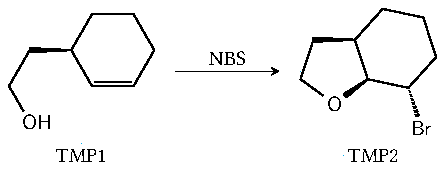
\includegraphics{scheme-tmp.ps}
  \end{document}
\end{example}

The tags now can be replaced with labels.  The result is shown in
figure~\ref{fig:scheme-tmp-tags-replaced}.
\begin{example}[compile,exe-with={--shell-escape},runs=1,float=htbp,caption={A scheme with
  temporary tags replaced with labels.\label{fig:scheme-tmp-tags-replaced}}]
  % code for figure 2 -- compiled with shell-escape enabled
  \documentclass{standalone}
  \usepackage{graphicx,auto-pst-pdf,chemnum}
  \begin{document}
    \replacecmpd{Alc}% replaces TMP1
    \replacecmpd{EtherBr}% replaces TMP2
    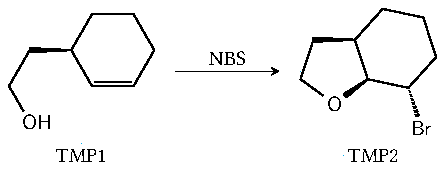
\includegraphics{scheme-tmp.ps}
  \end{document}
\end{example}

The replacement is done with the help of the \pkg{psfrag}
package~\cite{pkg:psfrag} and its \cs{psfrag} command.  For details on this
package and its command I refer to its documentation.

Although the examples don't do it the usage of \cs{replacecmpd} and the
corresponding graphic file should be placed inside a group (probably a
\env*{figure} or a \env*{scheme} environment) in order to keep the stepping of
the tag number local: this allows to use the same tags \code{TMP1},
\code{TMP2}, \ldots, in the next figure again.

As you can see the labels are printed sans serif.  This setting can of course
be changed.  The complete list of options is this:
\begin{options}
  \keybool{replace-auto}\Module{general}\Default{true}
    When set to true this adds an incremented integer to the replacement tag.
  \keyval{replace-tag}{text}\Module{general}\Default{TMP}
    The default replacement tag.
  \keyval{replace-tag-nr}{int}\Module{general}\Default{1}
    The\sinceversion{1.1} next number used by \cs{replacecmpd} when the
    default tag is used.
  \keyval{tag}{text}\Module{replace}\Default{TMP\meta{number}}
    The local replacement tag.  \meta{number} is incremented by one at each
    use and starts with \code{1}.  The starting number can be changed with the
    option \option{replace-tag-nr}.  The increment happens locally.
  \keyval{replace-style}{code}\Module{general}\Default{\cs*{sffamily}}
    Additional \TeX\ code that it placed before the \cs{cmpd} command in the
    replacement.
  \keyval{style}{code}\Module{replace}\Default{\cs*{sffamily}}
    Local additional \TeX\ code that it placed before the \cs{cmpd} command in
    the replacement.
  \keychoice{replace-pos}{\marg{\TeX\ pos}\marg{\ac{ps}
      pos}}\Module{general}\Default{bb}
    Options for \pkg{psfrag}'s \cs{psfrag}.
  \keychoice{pos}{\marg{\TeX\ pos}\marg{\ac{ps}
      pos}}\Module{replace}\Default{bb}
    Local options for \pkg{psfrag}'s \cs{psfrag}.  
\end{options}

If you have a scheme with arbitrary tabs like in
figure~\ref{fig:scheme-bla-tags} you can specify the \option{tag} option to
\cs{replacecmpd}.  Figure~\ref{fig:scheme-bla-tags-replaced} demonstrates
this.  It also demonstrates that you can of course use sublabels in the
\cs{replacecmpd} command.

\begin{example}[compile,exe-with={--shell-escape},runs=1,float=htbp,caption={A scheme with
  arbitrary tags.\label{fig:scheme-bla-tags}}]
  % code for figure 3
  \documentclass{standalone}
  \usepackage{graphicx,auto-pst-pdf}
  \begin{document}
    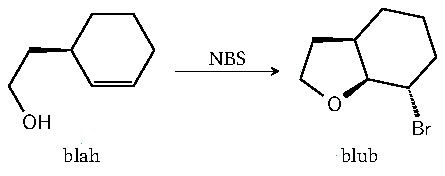
\includegraphics{scheme-bla.ps}
  \end{document}
\end{example}

If you don't want to use \code{TMP\meta{number}} as temporary tags but for
example \code{temp\meta{number}} you can change this with following option:
\begin{sourcecode}
  \setchemnum{replace-tag=temp}
\end{sourcecode}

The options \option{pos} and \option{replace-pos} refer to \cs{psfrag}'s
optional arguments which determine the positioning of the \TeX\ box with
respect to the \ac{ps} box that is replaced.  This is described in
\pkg{psfrag}'s documentation.

\begin{example}[compile,exe-with={--shell-escape},runs=1,float=htbp,caption={A scheme with
  arbitrary tags replaced with labels.\label{fig:scheme-bla-tags-replaced}}]
  % code for figure 4 -- compiled with shell-escape enabled
  \documentclass{standalone}
  \usepackage{graphicx,auto-pst-pdf,chemnum}
  \begin{document}
    \setchemnum{replace-style=\itshape}
    \replacecmpd[tag=blah]{main}% replaces blah
    \replacecmpd[tag=blub]{main.sub}% replaces blub
    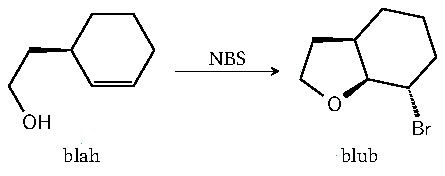
\includegraphics{scheme-bla.ps}
  \end{document}
\end{example}

\section{Changing the Input Markers}\label{sec:chang-input-mark}

In \chemnum's labels there are two markers (or three, actually) that can't be
part of a label name: the comma \code{,} and the dot \code{.}.  You can change
them with options:

\begin{options}
  \keyval{list-label-sep}{token}\Module{general}\Default{,}
    The marker that is used to split an input list of main labels.
  \keyval{sub-list-label-sep}{token}\Module{general}\Default{,}
    The marker that is used to split an input list of sublabels.
  \keyval{main-sub-sep}{token}\Module{general}\Default{.}
    The marker that divides sublabels from main labels.
\end{options}

\begin{example}[side-by-side]
  \setchemnum{
    main-sub-sep = ! ,
    list-label-sep = ;
  }
  \cmpd{a; b; c; e; g!two} \par
  \cmpd{q!one,two,three,four,five}
\end{example}

\section{Language Dependent Settings}\label{sec:lang-depend-sett}

A few settings of \chemnum\ depend on the language you chose with
\pkg{babel}~\cite{pkg:babel} or \pkg{polyglossia}~\cite{pkg:polyglossia}.
Those regard the list separators.  The language dependent strings are
translated with the help of the \pkg{translations}~\cite{pkg:translations}
package.  This package provides the means to define translations for strings
associated with identification keys.  \chemnum\ defines two strings. The
available languages and the corresponding translations of the two strings are
listed in table~\ref{tab:languages}. Note that both the comma or a leading
space as well as a trailing space are part of the translations.  To make this
obvious the relevant parts of the table are typeset in monotype and spaces are
represented by \code{\textvisiblespace}.

If you find your language missing or the translation to your language to be
wrong please write me an email and I'll add your language or fix the wrong
translation.

\begin{table}[htbp]
  \newcommand*\showlanguageentry[1]{%
    #1
    & \visualizespaces{\GetTranslationFor{#1}{chemnum-sep-two}}
    & \visualizespaces{\GetTranslationFor{#1}{chemnum-sep-last-two}}
  }
  \centering
  \caption{Available languages}
  \label{tab:languages}
  \begin{tabular}{l>{\ttfamily}l>{\ttfamily}l}
    \toprule
      \bfseries Language &
      \bfseries chemnum-sep-two &
      \bfseries chemnum-sep-last-two \\
    \midrule
      \showlanguageentry{English} \\
      \showlanguageentry{American} \\
      \showlanguageentry{German} \\
      \showlanguageentry{French} \\
      \showlanguageentry{Spanish} \\
      \showlanguageentry{Italian} \\
      \showlanguageentry{Catalan} \\
      \showlanguageentry{Portuguese} \\
      \showlanguageentry{Dutch} \\
      \showlanguageentry{Danish} \\
      \showlanguageentry{Swedish} \\
      \showlanguageentry{Finnish} \\
      \showlanguageentry{Norwegian} \\
    \bottomrule
  \end{tabular}
\end{table}

\section{Debugging Information}\label{sec:debugg-inform}

If you want information on the labels you have defined you can exploit the
following options:
\begin{options}
  \keychoice{log}{\default{true},false,silent,verbose}\Module{general}\Default{false}
    Determines how the declaration of the labels will be logged.  \code{false}
    means that no information is written to the \code{.log} file.  \code{true}
    means that basic information is written to the \code{.log} file when a
    label or a sublabel is declared.  \code{silent} is an alias of
    \code{true}.  \code{verbose} means that detailed information is written to
    the \code{.log} file when a label or a sublabel is declared.
  \keychoice{show-keys}{\default{true},false,def,ref}\Module{general}\Default{false}
    This option will write visual hints when a label is defined (choices
    \code{true} or \code{def}) or when a label is referenced (choices
    \code{true} or \code{ref}).
\end{options}

The option \option{log} will write information on a label to the \code{log}
file when a label is defined.  Depending on the choice (\code{true}, its alias
\code{silent}, or \code{verbose}) this will be only the main information or
detailed information including label properties.  The following code shows an
example when \keyis{log}{verbose}:
\begin{sourcecode}
  .................................................
  . chemnum info: defined new compound:
  .   ID = a
  .   internal number = 1
  .   label = 1
  .   pre label code = (
  .   post label code = )
  .   post main label code = 
  .   format = \bfseries 
  .................................................
\end{sourcecode}

The \option{show-keys} writes some visual information to the document itself:
\begin{example}
  \setchemnum{show-keys}
  \cmpd{a} and a bit later \cmpd{b}.
\end{example}
The last example shows the information when a label is referenced.  If a label
is newly declared information is written to the margin like for this label
with the \ac{id} \code{showkey}: \setchemnum{show-keys}\cmpd{showkey} that
again is referencend here: \cmpd{showkey}.

The option activates four commands:
\begin{commands}
  \command{cmpdshowdef}[\marg{\ac{id}}]
    Internal command used to display \meta{\ac{id}} of a newly defined compound
    label when the option \option{show-keys} is used.  The command is
    described in section~\ref{sec:debugg-inform}.
  \command{cmpdshowref}[\marg{\ac{id}}]
    Internal command used to display \meta{\ac{id}} of a referencing compound
    label when the option \option{show-keys} is used.  The command is
    described in section~\ref{sec:debugg-inform}.
  \command{subcmpdshowdef}[\marg{main \ac{id}}\marg{sub \ac{id}}]
    Internal command used to display \meta{main \ac{id}} and \meta{sub
      \ac{id}} of a newly defined subcompound label when the option
    \option{show-keys} is used.  The command is described in
    section~\ref{sec:debugg-inform}.
  \command{subcmpdshowref}[\marg{main \ac{id}}\marg{sub \ac{id}}]
    Internal command used to display \meta{main \ac{id}} and \meta{sub
      \ac{id}} of a referencing subcompound label when the option
    \option{show-keys} is used.  The command is described in
    section~\ref{sec:debugg-inform}.
\end{commands}
This means you can customize the appearance of the information by redefining
those commands.  The ones that show the definition use a \cs*{marginpar} in
their default definition.  This may cause them to disappear if issued
somewhere \cs*{marginpar} cannot be used.  The following shows an equivalent
definition with \cs*{marginnote} from the \pkg{marginnote}
package~\cite{pkg:marginnote}.  (This definition has another drawback: it
several \cs*{marginnote}s can print over one another if issued in the same
line.)

\begin{example}
  \renewcommand*\cmpdshowdef[1]{% /needs/ one mandatory argument
    \marginnote{\fbox{\normalfont\ttfamily#1}}}
  \renewcommand*\subcmpdshowdef[2]{% /needs/ two mandatory arguments
    \marginnote{\fbox{\normalfont\ttfamily#2 (#1)}}}
  a\cmpdshowdef{foo}\par
  b\cmpdshowref{foo}\par
  c\subcmpdshowdef{foo}{bar}\par
  d\subcmpdshowref{foo}{bar}
\end{example}

Actually there are two other commands you could redefine -- all four of the
above commands are defined in terms of them:
\begin{sourcecode}
  \NewDocumentCommand\cmpdshowdef{m}{\chemnumshowdef{#1}}
  \NewDocumentCommand\cmpdshowref{m}{\chemnumshowref{#1}}
  \NewDocumentCommand\subcmpdshowdef{mm}{\chemnumshowdef{#2 (#1)}}
  \NewDocumentCommand\subcmpdshowref{mm}{\chemnumshowref{#2}}
\end{sourcecode}

\end{document}


